\documentclass[twoside]{book}

% Packages required by doxygen
\usepackage{fixltx2e}
\usepackage{calc}
\usepackage{doxygen}
\usepackage[export]{adjustbox} % also loads graphicx
\usepackage{graphicx}
\usepackage[utf8]{inputenc}
\usepackage{makeidx}
\usepackage{multicol}
\usepackage{multirow}
\PassOptionsToPackage{warn}{textcomp}
\usepackage{textcomp}
\usepackage[nointegrals]{wasysym}
\usepackage[table]{xcolor}

% Font selection
\usepackage[T1]{fontenc}
\usepackage[scaled=.90]{helvet}
\usepackage{courier}
\usepackage{amssymb}
\usepackage{sectsty}
\renewcommand{\familydefault}{\sfdefault}
\allsectionsfont{%
  \fontseries{bc}\selectfont%
  \color{darkgray}%
}
\renewcommand{\DoxyLabelFont}{%
  \fontseries{bc}\selectfont%
  \color{darkgray}%
}
\newcommand{\+}{\discretionary{\mbox{\scriptsize$\hookleftarrow$}}{}{}}

% Page & text layout
\usepackage{geometry}
\geometry{%
  a4paper,%
  top=2.5cm,%
  bottom=2.5cm,%
  left=2.5cm,%
  right=2.5cm%
}
\tolerance=750
\hfuzz=15pt
\hbadness=750
\setlength{\emergencystretch}{15pt}
\setlength{\parindent}{0cm}
\setlength{\parskip}{3ex plus 2ex minus 2ex}
\makeatletter
\renewcommand{\paragraph}{%
  \@startsection{paragraph}{4}{0ex}{-1.0ex}{1.0ex}{%
    \normalfont\normalsize\bfseries\SS@parafont%
  }%
}
\renewcommand{\subparagraph}{%
  \@startsection{subparagraph}{5}{0ex}{-1.0ex}{1.0ex}{%
    \normalfont\normalsize\bfseries\SS@subparafont%
  }%
}
\makeatother

% Headers & footers
\usepackage{fancyhdr}
\pagestyle{fancyplain}
\fancyhead[LE]{\fancyplain{}{\bfseries\thepage}}
\fancyhead[CE]{\fancyplain{}{}}
\fancyhead[RE]{\fancyplain{}{\bfseries\leftmark}}
\fancyhead[LO]{\fancyplain{}{\bfseries\rightmark}}
\fancyhead[CO]{\fancyplain{}{}}
\fancyhead[RO]{\fancyplain{}{\bfseries\thepage}}
\fancyfoot[LE]{\fancyplain{}{}}
\fancyfoot[CE]{\fancyplain{}{}}
\fancyfoot[RE]{\fancyplain{}{\bfseries\scriptsize Generated by Doxygen }}
\fancyfoot[LO]{\fancyplain{}{\bfseries\scriptsize Generated by Doxygen }}
\fancyfoot[CO]{\fancyplain{}{}}
\fancyfoot[RO]{\fancyplain{}{}}
\renewcommand{\footrulewidth}{0.4pt}
\renewcommand{\chaptermark}[1]{%
  \markboth{#1}{}%
}
\renewcommand{\sectionmark}[1]{%
  \markright{\thesection\ #1}%
}

% Indices & bibliography
\usepackage{natbib}
\usepackage[titles]{tocloft}
\setcounter{tocdepth}{3}
\setcounter{secnumdepth}{5}
\makeindex

% Hyperlinks (required, but should be loaded last)
\usepackage{ifpdf}
\ifpdf
  \usepackage[pdftex,pagebackref=true]{hyperref}
\else
  \usepackage[ps2pdf,pagebackref=true]{hyperref}
\fi
\hypersetup{%
  colorlinks=true,%
  linkcolor=blue,%
  citecolor=blue,%
  unicode%
}

% Custom commands
\newcommand{\clearemptydoublepage}{%
  \newpage{\pagestyle{empty}\cleardoublepage}%
}

\usepackage{caption}
\captionsetup{labelsep=space,justification=centering,font={bf},singlelinecheck=off,skip=4pt,position=top}

%===== C O N T E N T S =====

\begin{document}

% Titlepage & ToC
\hypersetup{pageanchor=false,
             bookmarksnumbered=true,
             pdfencoding=unicode
            }
\pagenumbering{roman}
\begin{titlepage}
\vspace*{7cm}
\begin{center}%
{\Large My Project }\\
\vspace*{1cm}
{\large Generated by Doxygen 1.8.11}\\
\end{center}
\end{titlepage}
\clearemptydoublepage
\tableofcontents
\clearemptydoublepage
\pagenumbering{arabic}
\hypersetup{pageanchor=true}

%--- Begin generated contents ---
\chapter{Hierarchical Index}
\section{Class Hierarchy}
This inheritance list is sorted roughly, but not completely, alphabetically\+:\begin{DoxyCompactList}
\item \contentsline{section}{Fruit}{\pageref{classFruit}}{}
\begin{DoxyCompactList}
\item \contentsline{section}{Apple}{\pageref{classApple}}{}
\item \contentsline{section}{Grape}{\pageref{classGrape}}{}
\item \contentsline{section}{Orange}{\pageref{classOrange}}{}
\end{DoxyCompactList}
\item \contentsline{section}{List}{\pageref{classList}}{}
\item \contentsline{section}{List\+:\+:Node}{\pageref{structList_1_1Node}}{}
\end{DoxyCompactList}

\chapter{Class Index}
\section{Class List}
Here are the classes, structs, unions and interfaces with brief descriptions\+:\begin{DoxyCompactList}
\item\contentsline{section}{\hyperlink{structnode}{node} }{\pageref{structnode}}{}
\item\contentsline{section}{\hyperlink{structnode1}{node1} }{\pageref{structnode1}}{}
\item\contentsline{section}{\hyperlink{structnode__info}{node\+\_\+info} }{\pageref{structnode__info}}{}
\end{DoxyCompactList}

\chapter{File Index}
\section{File List}
Here is a list of all files with brief descriptions\+:\begin{DoxyCompactList}
\item\contentsline{section}{\hyperlink{Lab1_8c}{Lab1.\+c} }{\pageref{Lab1_8c}}{}
\end{DoxyCompactList}

\chapter{Class Documentation}
\hypertarget{classCore}{}\section{Core Class Reference}
\label{classCore}\index{Core@{Core}}


Inheritance diagram for Core\+:
\nopagebreak
\begin{figure}[H]
\begin{center}
\leavevmode
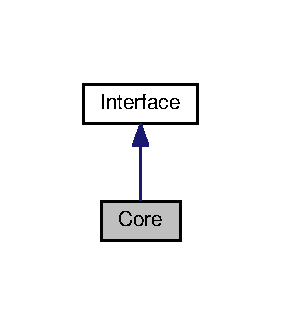
\includegraphics[width=135pt]{classCore__inherit__graph}
\end{center}
\end{figure}


Collaboration diagram for Core\+:
\nopagebreak
\begin{figure}[H]
\begin{center}
\leavevmode
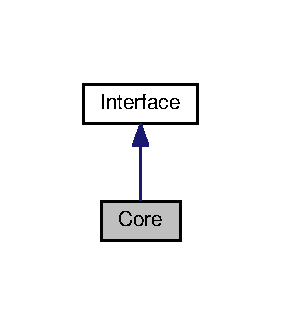
\includegraphics[width=135pt]{classCore__coll__graph}
\end{center}
\end{figure}
\subsection*{Public Member Functions}
\begin{DoxyCompactItemize}
\item 
\hyperlink{classCore_a776f8c46504b14183883c6273f93eaed}{$\sim$\+Core} ()
\item 
virtual void \hyperlink{classCore_a895d6310ade8397dfc64461ac55a80a9}{write} (std\+::string \&text) override
\end{DoxyCompactItemize}


\subsection{Constructor \& Destructor Documentation}
\index{Core@{Core}!````~Core@{$\sim$\+Core}}
\index{````~Core@{$\sim$\+Core}!Core@{Core}}
\subsubsection[{\texorpdfstring{$\sim$\+Core()}{~Core()}}]{\setlength{\rightskip}{0pt plus 5cm}Core\+::$\sim$\+Core (
\begin{DoxyParamCaption}
{}
\end{DoxyParamCaption}
)\hspace{0.3cm}{\ttfamily [inline]}}\hypertarget{classCore_a776f8c46504b14183883c6273f93eaed}{}\label{classCore_a776f8c46504b14183883c6273f93eaed}

\begin{DoxyCode}
13 \{std::cout << \textcolor{stringliteral}{"Core destructor called.\(\backslash\)n"};\}
\end{DoxyCode}


\subsection{Member Function Documentation}
\index{Core@{Core}!write@{write}}
\index{write@{write}!Core@{Core}}
\subsubsection[{\texorpdfstring{write(std\+::string \&text) override}{write(std::string &text) override}}]{\setlength{\rightskip}{0pt plus 5cm}virtual void Core\+::write (
\begin{DoxyParamCaption}
\item[{std\+::string \&}]{text}
\end{DoxyParamCaption}
)\hspace{0.3cm}{\ttfamily [inline]}, {\ttfamily [override]}, {\ttfamily [virtual]}}\hypertarget{classCore_a895d6310ade8397dfc64461ac55a80a9}{}\label{classCore_a895d6310ade8397dfc64461ac55a80a9}


Implements \hyperlink{classInterface_a8a27e796f257a35b468c06579af48d85}{Interface}.


\begin{DoxyCode}
14 \{\};  \textcolor{comment}{// Do nothing.}
\end{DoxyCode}


The documentation for this class was generated from the following file\+:\begin{DoxyCompactItemize}
\item 
\hyperlink{Decorator2_8cpp}{Decorator2.\+cpp}\end{DoxyCompactItemize}

\hypertarget{classDecorator}{}\section{Decorator Class Reference}
\label{classDecorator}\index{Decorator@{Decorator}}


Inheritance diagram for Decorator\+:
\nopagebreak
\begin{figure}[H]
\begin{center}
\leavevmode
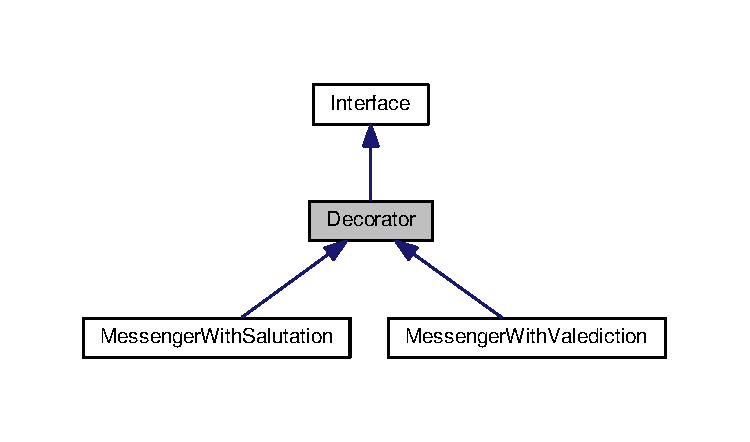
\includegraphics[width=350pt]{classDecorator__inherit__graph}
\end{center}
\end{figure}


Collaboration diagram for Decorator\+:
\nopagebreak
\begin{figure}[H]
\begin{center}
\leavevmode
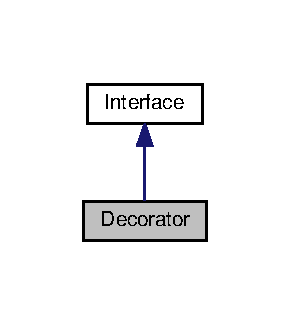
\includegraphics[width=139pt]{classDecorator__coll__graph}
\end{center}
\end{figure}
\subsection*{Public Member Functions}
\begin{DoxyCompactItemize}
\item 
\hyperlink{classDecorator_aee6cdf11333827f13ea5b5384ad5af88}{Decorator} (std\+::unique\+\_\+ptr$<$ \hyperlink{classInterface}{Interface} $>$ c)
\item 
virtual void \hyperlink{classDecorator_ae5cad6daee450fb5eaa2b1cad6a0dd45}{write} (std\+::string \&text) override
\end{DoxyCompactItemize}
\subsection*{Private Attributes}
\begin{DoxyCompactItemize}
\item 
std\+::unique\+\_\+ptr$<$ \hyperlink{classInterface}{Interface} $>$ \hyperlink{classDecorator_a97d246b8a8a01f52ff6cd8f53aac1727}{interface}
\end{DoxyCompactItemize}


\subsection{Constructor \& Destructor Documentation}
\index{Decorator@{Decorator}!Decorator@{Decorator}}
\index{Decorator@{Decorator}!Decorator@{Decorator}}
\subsubsection[{\texorpdfstring{Decorator(std\+::unique\+\_\+ptr$<$ Interface $>$ c)}{Decorator(std::unique_ptr< Interface > c)}}]{\setlength{\rightskip}{0pt plus 5cm}Decorator\+::\+Decorator (
\begin{DoxyParamCaption}
\item[{std\+::unique\+\_\+ptr$<$ {\bf Interface} $>$}]{c}
\end{DoxyParamCaption}
)\hspace{0.3cm}{\ttfamily [inline]}}\hypertarget{classDecorator_aee6cdf11333827f13ea5b5384ad5af88}{}\label{classDecorator_aee6cdf11333827f13ea5b5384ad5af88}

\begin{DoxyCode}
21 \{\textcolor{keyword}{interface }= std::move(c);\}
\end{DoxyCode}


\subsection{Member Function Documentation}
\index{Decorator@{Decorator}!write@{write}}
\index{write@{write}!Decorator@{Decorator}}
\subsubsection[{\texorpdfstring{write(std\+::string \&text) override}{write(std::string &text) override}}]{\setlength{\rightskip}{0pt plus 5cm}virtual void Decorator\+::write (
\begin{DoxyParamCaption}
\item[{std\+::string \&}]{text}
\end{DoxyParamCaption}
)\hspace{0.3cm}{\ttfamily [inline]}, {\ttfamily [override]}, {\ttfamily [virtual]}}\hypertarget{classDecorator_ae5cad6daee450fb5eaa2b1cad6a0dd45}{}\label{classDecorator_ae5cad6daee450fb5eaa2b1cad6a0dd45}


Implements \hyperlink{classInterface_a8a27e796f257a35b468c06579af48d85}{Interface}.



Reimplemented in \hyperlink{classMessengerWithValediction_a93f7e5fc32a11b58b3c57b54544ec8a2}{Messenger\+With\+Valediction}, and \hyperlink{classMessengerWithSalutation_aed33b1b35b9c5c24f80a3e898aed2487}{Messenger\+With\+Salutation}.


\begin{DoxyCode}
22 \{\hyperlink{classDecorator_a97d246b8a8a01f52ff6cd8f53aac1727}{interface}->write(text);\}
\end{DoxyCode}


\subsection{Member Data Documentation}
\index{Decorator@{Decorator}!interface@{interface}}
\index{interface@{interface}!Decorator@{Decorator}}
\subsubsection[{\texorpdfstring{interface}{interface}}]{\setlength{\rightskip}{0pt plus 5cm}std\+::unique\+\_\+ptr$<${\bf Interface}$>$ Decorator\+::interface\hspace{0.3cm}{\ttfamily [private]}}\hypertarget{classDecorator_a97d246b8a8a01f52ff6cd8f53aac1727}{}\label{classDecorator_a97d246b8a8a01f52ff6cd8f53aac1727}


The documentation for this class was generated from the following file\+:\begin{DoxyCompactItemize}
\item 
\hyperlink{Decorator2_8cpp}{Decorator2.\+cpp}\end{DoxyCompactItemize}

\hypertarget{classInterface}{}\section{Interface Class Reference}
\label{classInterface}\index{Interface@{Interface}}


Inheritance diagram for Interface\+:
\nopagebreak
\begin{figure}[H]
\begin{center}
\leavevmode
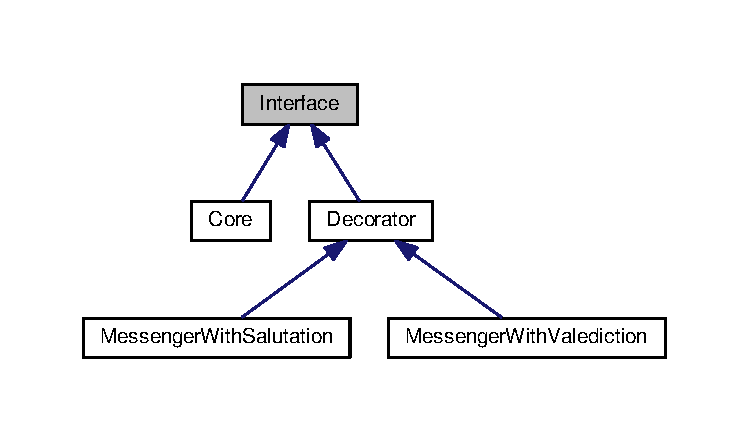
\includegraphics[width=350pt]{classInterface__inherit__graph}
\end{center}
\end{figure}
\subsection*{Public Member Functions}
\begin{DoxyCompactItemize}
\item 
virtual \hyperlink{classInterface_a67eca71a4ef8d28dc959dd495e2b2b59}{$\sim$\+Interface} ()
\item 
virtual void \hyperlink{classInterface_a8a27e796f257a35b468c06579af48d85}{write} (std\+::string \&)=0
\end{DoxyCompactItemize}


\subsection{Constructor \& Destructor Documentation}
\index{Interface@{Interface}!````~Interface@{$\sim$\+Interface}}
\index{````~Interface@{$\sim$\+Interface}!Interface@{Interface}}
\subsubsection[{\texorpdfstring{$\sim$\+Interface()}{~Interface()}}]{\setlength{\rightskip}{0pt plus 5cm}virtual Interface\+::$\sim$\+Interface (
\begin{DoxyParamCaption}
{}
\end{DoxyParamCaption}
)\hspace{0.3cm}{\ttfamily [inline]}, {\ttfamily [virtual]}}\hypertarget{classInterface_a67eca71a4ef8d28dc959dd495e2b2b59}{}\label{classInterface_a67eca71a4ef8d28dc959dd495e2b2b59}

\begin{DoxyCode}
7 \{ \}
\end{DoxyCode}


Here is the call graph for this function\+:
\nopagebreak
\begin{figure}[H]
\begin{center}
\leavevmode
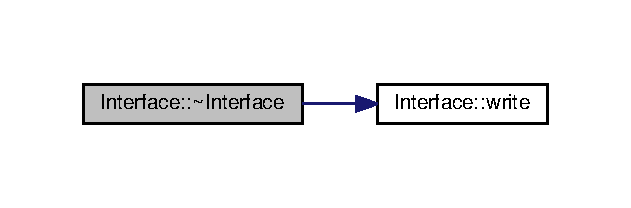
\includegraphics[width=303pt]{classInterface_a67eca71a4ef8d28dc959dd495e2b2b59_cgraph}
\end{center}
\end{figure}




\subsection{Member Function Documentation}
\index{Interface@{Interface}!write@{write}}
\index{write@{write}!Interface@{Interface}}
\subsubsection[{\texorpdfstring{write(std\+::string \&)=0}{write(std::string &)=0}}]{\setlength{\rightskip}{0pt plus 5cm}virtual void Interface\+::write (
\begin{DoxyParamCaption}
\item[{std\+::string \&}]{}
\end{DoxyParamCaption}
)\hspace{0.3cm}{\ttfamily [pure virtual]}}\hypertarget{classInterface_a8a27e796f257a35b468c06579af48d85}{}\label{classInterface_a8a27e796f257a35b468c06579af48d85}


Implemented in \hyperlink{classMessengerWithValediction_a93f7e5fc32a11b58b3c57b54544ec8a2}{Messenger\+With\+Valediction}, \hyperlink{classMessengerWithSalutation_aed33b1b35b9c5c24f80a3e898aed2487}{Messenger\+With\+Salutation}, \hyperlink{classDecorator_ae5cad6daee450fb5eaa2b1cad6a0dd45}{Decorator}, and \hyperlink{classCore_a895d6310ade8397dfc64461ac55a80a9}{Core}.



The documentation for this class was generated from the following file\+:\begin{DoxyCompactItemize}
\item 
\hyperlink{Decorator2_8cpp}{Decorator2.\+cpp}\end{DoxyCompactItemize}

\hypertarget{classMessengerWithSalutation}{}\section{Messenger\+With\+Salutation Class Reference}
\label{classMessengerWithSalutation}\index{Messenger\+With\+Salutation@{Messenger\+With\+Salutation}}


Inheritance diagram for Messenger\+With\+Salutation\+:
\nopagebreak
\begin{figure}[H]
\begin{center}
\leavevmode
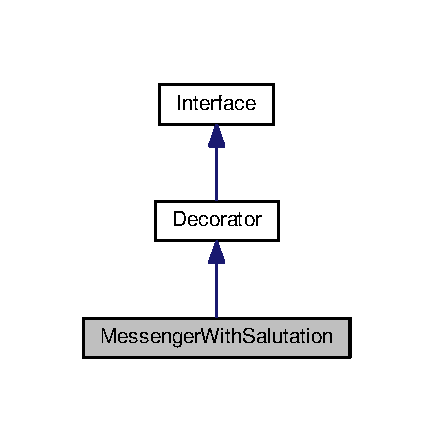
\includegraphics[width=208pt]{classMessengerWithSalutation__inherit__graph}
\end{center}
\end{figure}


Collaboration diagram for Messenger\+With\+Salutation\+:
\nopagebreak
\begin{figure}[H]
\begin{center}
\leavevmode
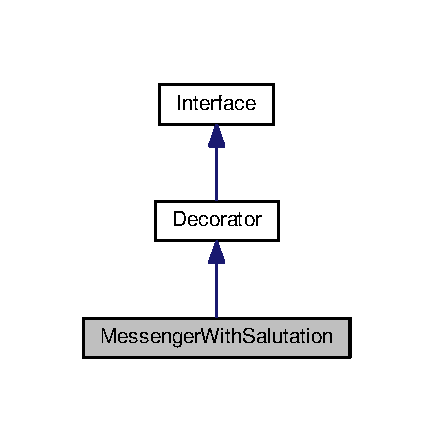
\includegraphics[width=208pt]{classMessengerWithSalutation__coll__graph}
\end{center}
\end{figure}
\subsection*{Public Member Functions}
\begin{DoxyCompactItemize}
\item 
\hyperlink{classMessengerWithSalutation_a6ec1cb0e7c58771265dfc20f1d75573a}{Messenger\+With\+Salutation} (std\+::unique\+\_\+ptr$<$ \hyperlink{classInterface}{Interface} $>$ c, const std\+::string \&str)
\item 
\hyperlink{classMessengerWithSalutation_ab98288095a6f7e7ddd768a5defab7f31}{$\sim$\+Messenger\+With\+Salutation} ()
\item 
virtual void \hyperlink{classMessengerWithSalutation_aed33b1b35b9c5c24f80a3e898aed2487}{write} (std\+::string \&text) override
\end{DoxyCompactItemize}
\subsection*{Private Attributes}
\begin{DoxyCompactItemize}
\item 
std\+::string \hyperlink{classMessengerWithSalutation_af3a570c7b7a40656b029803aa8419c43}{salutation}
\end{DoxyCompactItemize}


\subsection{Constructor \& Destructor Documentation}
\index{Messenger\+With\+Salutation@{Messenger\+With\+Salutation}!Messenger\+With\+Salutation@{Messenger\+With\+Salutation}}
\index{Messenger\+With\+Salutation@{Messenger\+With\+Salutation}!Messenger\+With\+Salutation@{Messenger\+With\+Salutation}}
\subsubsection[{\texorpdfstring{Messenger\+With\+Salutation(std\+::unique\+\_\+ptr$<$ Interface $>$ c, const std\+::string \&str)}{MessengerWithSalutation(std::unique_ptr< Interface > c, const std::string &str)}}]{\setlength{\rightskip}{0pt plus 5cm}Messenger\+With\+Salutation\+::\+Messenger\+With\+Salutation (
\begin{DoxyParamCaption}
\item[{std\+::unique\+\_\+ptr$<$ {\bf Interface} $>$}]{c, }
\item[{const std\+::string \&}]{str}
\end{DoxyParamCaption}
)\hspace{0.3cm}{\ttfamily [inline]}}\hypertarget{classMessengerWithSalutation_a6ec1cb0e7c58771265dfc20f1d75573a}{}\label{classMessengerWithSalutation_a6ec1cb0e7c58771265dfc20f1d75573a}

\begin{DoxyCode}
29 : \hyperlink{classDecorator_aee6cdf11333827f13ea5b5384ad5af88}{Decorator}(std::move(c)), \hyperlink{classMessengerWithSalutation_af3a570c7b7a40656b029803aa8419c43}{salutation}(str) \{\}
\end{DoxyCode}
\index{Messenger\+With\+Salutation@{Messenger\+With\+Salutation}!````~Messenger\+With\+Salutation@{$\sim$\+Messenger\+With\+Salutation}}
\index{````~Messenger\+With\+Salutation@{$\sim$\+Messenger\+With\+Salutation}!Messenger\+With\+Salutation@{Messenger\+With\+Salutation}}
\subsubsection[{\texorpdfstring{$\sim$\+Messenger\+With\+Salutation()}{~MessengerWithSalutation()}}]{\setlength{\rightskip}{0pt plus 5cm}Messenger\+With\+Salutation\+::$\sim$\+Messenger\+With\+Salutation (
\begin{DoxyParamCaption}
{}
\end{DoxyParamCaption}
)\hspace{0.3cm}{\ttfamily [inline]}}\hypertarget{classMessengerWithSalutation_ab98288095a6f7e7ddd768a5defab7f31}{}\label{classMessengerWithSalutation_ab98288095a6f7e7ddd768a5defab7f31}

\begin{DoxyCode}
30 \{std::cout << \textcolor{stringliteral}{"Messenger destructor called.\(\backslash\)n"};\}
\end{DoxyCode}


\subsection{Member Function Documentation}
\index{Messenger\+With\+Salutation@{Messenger\+With\+Salutation}!write@{write}}
\index{write@{write}!Messenger\+With\+Salutation@{Messenger\+With\+Salutation}}
\subsubsection[{\texorpdfstring{write(std\+::string \&text) override}{write(std::string &text) override}}]{\setlength{\rightskip}{0pt plus 5cm}virtual void Messenger\+With\+Salutation\+::write (
\begin{DoxyParamCaption}
\item[{std\+::string \&}]{text}
\end{DoxyParamCaption}
)\hspace{0.3cm}{\ttfamily [inline]}, {\ttfamily [override]}, {\ttfamily [virtual]}}\hypertarget{classMessengerWithSalutation_aed33b1b35b9c5c24f80a3e898aed2487}{}\label{classMessengerWithSalutation_aed33b1b35b9c5c24f80a3e898aed2487}


Reimplemented from \hyperlink{classDecorator_ae5cad6daee450fb5eaa2b1cad6a0dd45}{Decorator}.


\begin{DoxyCode}
31                                                       \{
32             text = \hyperlink{classMessengerWithSalutation_af3a570c7b7a40656b029803aa8419c43}{salutation} + \textcolor{stringliteral}{"\(\backslash\)n\(\backslash\)n"} + text;
33             \hyperlink{classDecorator_ae5cad6daee450fb5eaa2b1cad6a0dd45}{Decorator::write}(text);
34         \}
\end{DoxyCode}


Here is the call graph for this function\+:
\nopagebreak
\begin{figure}[H]
\begin{center}
\leavevmode
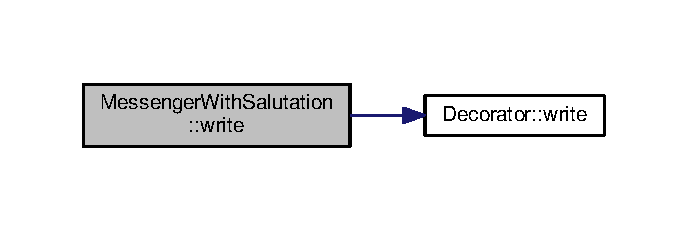
\includegraphics[width=330pt]{classMessengerWithSalutation_aed33b1b35b9c5c24f80a3e898aed2487_cgraph}
\end{center}
\end{figure}




\subsection{Member Data Documentation}
\index{Messenger\+With\+Salutation@{Messenger\+With\+Salutation}!salutation@{salutation}}
\index{salutation@{salutation}!Messenger\+With\+Salutation@{Messenger\+With\+Salutation}}
\subsubsection[{\texorpdfstring{salutation}{salutation}}]{\setlength{\rightskip}{0pt plus 5cm}std\+::string Messenger\+With\+Salutation\+::salutation\hspace{0.3cm}{\ttfamily [private]}}\hypertarget{classMessengerWithSalutation_af3a570c7b7a40656b029803aa8419c43}{}\label{classMessengerWithSalutation_af3a570c7b7a40656b029803aa8419c43}


The documentation for this class was generated from the following file\+:\begin{DoxyCompactItemize}
\item 
\hyperlink{Decorator2_8cpp}{Decorator2.\+cpp}\end{DoxyCompactItemize}

\hypertarget{classMessengerWithValediction}{}\section{Messenger\+With\+Valediction Class Reference}
\label{classMessengerWithValediction}\index{Messenger\+With\+Valediction@{Messenger\+With\+Valediction}}


Inheritance diagram for Messenger\+With\+Valediction\+:
\nopagebreak
\begin{figure}[H]
\begin{center}
\leavevmode
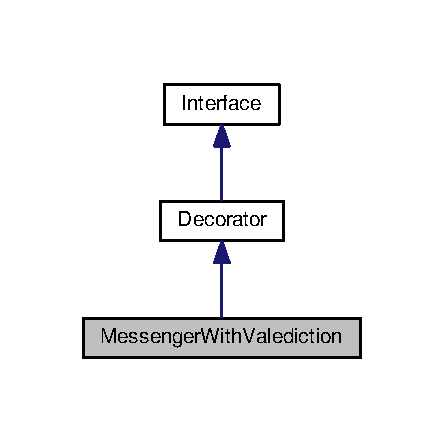
\includegraphics[width=213pt]{classMessengerWithValediction__inherit__graph}
\end{center}
\end{figure}


Collaboration diagram for Messenger\+With\+Valediction\+:
\nopagebreak
\begin{figure}[H]
\begin{center}
\leavevmode
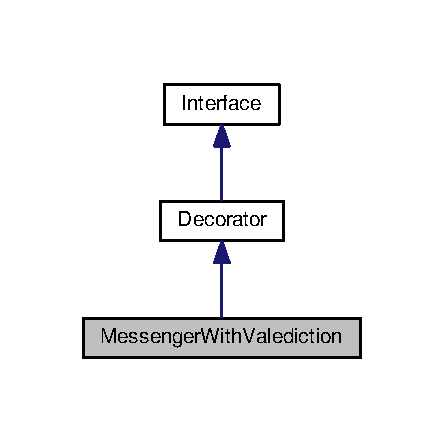
\includegraphics[width=213pt]{classMessengerWithValediction__coll__graph}
\end{center}
\end{figure}
\subsection*{Public Member Functions}
\begin{DoxyCompactItemize}
\item 
\hyperlink{classMessengerWithValediction_a15972054fa38938f0213b3f0749a6148}{Messenger\+With\+Valediction} (std\+::unique\+\_\+ptr$<$ \hyperlink{classInterface}{Interface} $>$ c, const std\+::string \&str)
\item 
\hyperlink{classMessengerWithValediction_a9205d11f633fdf1099f62436aa638a1e}{$\sim$\+Messenger\+With\+Valediction} ()
\item 
virtual void \hyperlink{classMessengerWithValediction_a93f7e5fc32a11b58b3c57b54544ec8a2}{write} (std\+::string \&text) override
\end{DoxyCompactItemize}
\subsection*{Private Attributes}
\begin{DoxyCompactItemize}
\item 
std\+::string \hyperlink{classMessengerWithValediction_ad8c759fc057a3b7d2331ec6a84a38895}{valediction}
\end{DoxyCompactItemize}


\subsection{Constructor \& Destructor Documentation}
\index{Messenger\+With\+Valediction@{Messenger\+With\+Valediction}!Messenger\+With\+Valediction@{Messenger\+With\+Valediction}}
\index{Messenger\+With\+Valediction@{Messenger\+With\+Valediction}!Messenger\+With\+Valediction@{Messenger\+With\+Valediction}}
\subsubsection[{\texorpdfstring{Messenger\+With\+Valediction(std\+::unique\+\_\+ptr$<$ Interface $>$ c, const std\+::string \&str)}{MessengerWithValediction(std::unique_ptr< Interface > c, const std::string &str)}}]{\setlength{\rightskip}{0pt plus 5cm}Messenger\+With\+Valediction\+::\+Messenger\+With\+Valediction (
\begin{DoxyParamCaption}
\item[{std\+::unique\+\_\+ptr$<$ {\bf Interface} $>$}]{c, }
\item[{const std\+::string \&}]{str}
\end{DoxyParamCaption}
)\hspace{0.3cm}{\ttfamily [inline]}}\hypertarget{classMessengerWithValediction_a15972054fa38938f0213b3f0749a6148}{}\label{classMessengerWithValediction_a15972054fa38938f0213b3f0749a6148}

\begin{DoxyCode}
41 : \hyperlink{classDecorator_aee6cdf11333827f13ea5b5384ad5af88}{Decorator}(std::move(c)), \hyperlink{classMessengerWithValediction_ad8c759fc057a3b7d2331ec6a84a38895}{valediction}(str) \{\}
\end{DoxyCode}
\index{Messenger\+With\+Valediction@{Messenger\+With\+Valediction}!````~Messenger\+With\+Valediction@{$\sim$\+Messenger\+With\+Valediction}}
\index{````~Messenger\+With\+Valediction@{$\sim$\+Messenger\+With\+Valediction}!Messenger\+With\+Valediction@{Messenger\+With\+Valediction}}
\subsubsection[{\texorpdfstring{$\sim$\+Messenger\+With\+Valediction()}{~MessengerWithValediction()}}]{\setlength{\rightskip}{0pt plus 5cm}Messenger\+With\+Valediction\+::$\sim$\+Messenger\+With\+Valediction (
\begin{DoxyParamCaption}
{}
\end{DoxyParamCaption}
)\hspace{0.3cm}{\ttfamily [inline]}}\hypertarget{classMessengerWithValediction_a9205d11f633fdf1099f62436aa638a1e}{}\label{classMessengerWithValediction_a9205d11f633fdf1099f62436aa638a1e}

\begin{DoxyCode}
42 \{std::cout << \textcolor{stringliteral}{"MessengerWithValediction destructor called.\(\backslash\)n"};\}
\end{DoxyCode}


\subsection{Member Function Documentation}
\index{Messenger\+With\+Valediction@{Messenger\+With\+Valediction}!write@{write}}
\index{write@{write}!Messenger\+With\+Valediction@{Messenger\+With\+Valediction}}
\subsubsection[{\texorpdfstring{write(std\+::string \&text) override}{write(std::string &text) override}}]{\setlength{\rightskip}{0pt plus 5cm}virtual void Messenger\+With\+Valediction\+::write (
\begin{DoxyParamCaption}
\item[{std\+::string \&}]{text}
\end{DoxyParamCaption}
)\hspace{0.3cm}{\ttfamily [inline]}, {\ttfamily [override]}, {\ttfamily [virtual]}}\hypertarget{classMessengerWithValediction_a93f7e5fc32a11b58b3c57b54544ec8a2}{}\label{classMessengerWithValediction_a93f7e5fc32a11b58b3c57b54544ec8a2}


Reimplemented from \hyperlink{classDecorator_ae5cad6daee450fb5eaa2b1cad6a0dd45}{Decorator}.


\begin{DoxyCode}
43                                                       \{
44             \hyperlink{classDecorator_ae5cad6daee450fb5eaa2b1cad6a0dd45}{Decorator::write}(text);
45             text += \textcolor{stringliteral}{"\(\backslash\)n\(\backslash\)n"} + \hyperlink{classMessengerWithValediction_ad8c759fc057a3b7d2331ec6a84a38895}{valediction};
46         \}
\end{DoxyCode}


Here is the call graph for this function\+:
\nopagebreak
\begin{figure}[H]
\begin{center}
\leavevmode
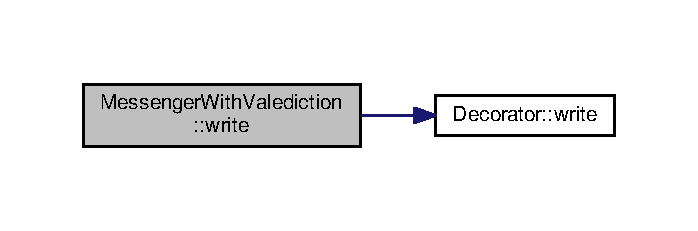
\includegraphics[width=335pt]{classMessengerWithValediction_a93f7e5fc32a11b58b3c57b54544ec8a2_cgraph}
\end{center}
\end{figure}




\subsection{Member Data Documentation}
\index{Messenger\+With\+Valediction@{Messenger\+With\+Valediction}!valediction@{valediction}}
\index{valediction@{valediction}!Messenger\+With\+Valediction@{Messenger\+With\+Valediction}}
\subsubsection[{\texorpdfstring{valediction}{valediction}}]{\setlength{\rightskip}{0pt plus 5cm}std\+::string Messenger\+With\+Valediction\+::valediction\hspace{0.3cm}{\ttfamily [private]}}\hypertarget{classMessengerWithValediction_ad8c759fc057a3b7d2331ec6a84a38895}{}\label{classMessengerWithValediction_ad8c759fc057a3b7d2331ec6a84a38895}


The documentation for this class was generated from the following file\+:\begin{DoxyCompactItemize}
\item 
\hyperlink{Decorator2_8cpp}{Decorator2.\+cpp}\end{DoxyCompactItemize}

\chapter{File Documentation}
\hypertarget{Decorator2_8cpp}{}\section{Decorator2.\+cpp File Reference}
\label{Decorator2_8cpp}\index{Decorator2.\+cpp@{Decorator2.\+cpp}}
{\ttfamily \#include $<$iostream$>$}\\*
{\ttfamily \#include $<$string$>$}\\*
{\ttfamily \#include $<$memory$>$}\\*
Include dependency graph for Decorator2.\+cpp\+:
\nopagebreak
\begin{figure}[H]
\begin{center}
\leavevmode
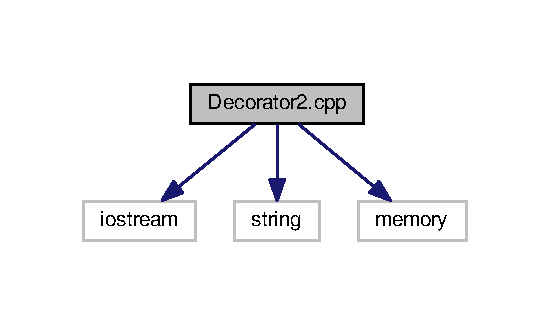
\includegraphics[width=264pt]{Decorator2_8cpp__incl}
\end{center}
\end{figure}
\subsection*{Classes}
\begin{DoxyCompactItemize}
\item 
class \hyperlink{classInterface}{Interface}
\item 
class \hyperlink{classCore}{Core}
\item 
class \hyperlink{classDecorator}{Decorator}
\item 
class \hyperlink{classMessengerWithSalutation}{Messenger\+With\+Salutation}
\item 
class \hyperlink{classMessengerWithValediction}{Messenger\+With\+Valediction}
\end{DoxyCompactItemize}
\subsection*{Functions}
\begin{DoxyCompactItemize}
\item 
int \hyperlink{Decorator2_8cpp_ae66f6b31b5ad750f1fe042a706a4e3d4}{main} ()
\end{DoxyCompactItemize}


\subsection{Function Documentation}
\index{Decorator2.\+cpp@{Decorator2.\+cpp}!main@{main}}
\index{main@{main}!Decorator2.\+cpp@{Decorator2.\+cpp}}
\subsubsection[{\texorpdfstring{main()}{main()}}]{\setlength{\rightskip}{0pt plus 5cm}int main (
\begin{DoxyParamCaption}
{}
\end{DoxyParamCaption}
)}\hypertarget{Decorator2_8cpp_ae66f6b31b5ad750f1fe042a706a4e3d4}{}\label{Decorator2_8cpp_ae66f6b31b5ad750f1fe042a706a4e3d4}

\begin{DoxyCode}
49            \{
50     \textcolor{keyword}{const} std::string salutation = \textcolor{stringliteral}{"Greetings,"};
51     \textcolor{keyword}{const} std::string valediction = \textcolor{stringliteral}{"Sincerly, Andy"};
52     std::string message1 = \textcolor{stringliteral}{"This message is not decorated."};
53     std::string message2 = \textcolor{stringliteral}{"This message is decorated with a salutation."};
54     std::string message3 = \textcolor{stringliteral}{"This message is decorated with a valediction."};
55     std::string message4 = \textcolor{stringliteral}{"This message is decorated with a salutation and a valediction."};
56 
57     std::unique\_ptr<Interface> messenger1 = std::make\_unique<Core>();
58     std::unique\_ptr<Interface> messenger2 = std::make\_unique<MessengerWithSalutation> (
      std::make\_unique<Core>(), salutation);
59     std::unique\_ptr<Interface> messenger3 = std::make\_unique<MessengerWithValediction> (
      std::make\_unique<Core>(), valediction);
60     std::unique\_ptr<Interface> messenger4 = std::make\_unique<MessengerWithValediction> (
      std::make\_unique<MessengerWithSalutation>
61                                           (std::make\_unique<Core>(), salutation), valediction);
62     
63     messenger1->write(message1);
64     std::cout << message1 << \textcolor{charliteral}{'\(\backslash\)n'};
65     std::cout << \textcolor{stringliteral}{"\(\backslash\)n------------------------------\(\backslash\)n\(\backslash\)n"};
66 
67     messenger2->write(message2);
68     std::cout << message2 << \textcolor{charliteral}{'\(\backslash\)n'};
69     std::cout << \textcolor{stringliteral}{"\(\backslash\)n------------------------------\(\backslash\)n\(\backslash\)n"};
70 
71     messenger3->write(message3);
72     std::cout << message3 << \textcolor{charliteral}{'\(\backslash\)n'};
73     std::cout << \textcolor{stringliteral}{"\(\backslash\)n------------------------------\(\backslash\)n\(\backslash\)n"};
74 
75     messenger4->write(message4);
76     std::cout << message4 << \textcolor{charliteral}{'\(\backslash\)n'};
77     std::cout << \textcolor{stringliteral}{"\(\backslash\)n------------------------------\(\backslash\)n\(\backslash\)n"};
78 \}\end{DoxyCode}

%--- End generated contents ---

% Index
\backmatter
\newpage
\phantomsection
\clearemptydoublepage
\addcontentsline{toc}{chapter}{Index}
\printindex

\end{document}
